%%%%%%%%%%%%%%%%%%%%%%%%%%%%%%%%%%%%%%%%%%%%%%%
%
% Template per Elaborato di Laurea
% DISI - Dipartimento di Ingegneria e Scienza dell’Informazione
%
% update 2015-09-10
%
% Per la generazione corretta del 
% pdflatex nome_file.tex
% bibtex nome_file.aux
% pdflatex nome_file.tex
% pdflatex nome_file.tex
%
%%%%%%%%%%%%%%%%%%%%%%%%%%%%%%%%%%%%%%%%%%%%%%%

% formato FRONTE RETRO
\documentclass[epsfig,a4paper,11pt,titlepage,twoside,openany]{book}
\usepackage{epsfig}
\usepackage{plain}
\usepackage{setspace}
\usepackage[paperheight=29.7cm,paperwidth=21cm,outer=1.5cm,inner=2.5cm,top=2cm,bottom=2cm]{geometry} % per definizione layout
\usepackage{titlesec} % per formato custom dei titoli dei capitoli
\usepackage{listings}
\usepackage{xcolor}



%%%%%%%%%%%%%%
% supporto lettere accentate
%
%\usepackage[latin1]{inputenc} % per Windows;
\usepackage[utf8x]{inputenc} % per Linux (richiede il pacchetto unicode);
%\usepackage[applemac]{inputenc} % per Mac.

\singlespacing

\usepackage[italian]{babel}

\begin{document}
%%%%%%%%%%%%%%%%%%%%%%%%%%%%%%%%%%%%%%%%%%%%%%%%%%%%%%%%%%%%%%%%%%%%%%%%%
  
  % nessuna numerazione
  \pagenumbering{gobble} 
  \pagestyle{plain}

\thispagestyle{empty}

\begin{center}
  \begin{figure}[h!]
    \centerline{
\psfig{file=logo/marchio_unitrento_colore_it_202002.eps,width=0.6\textwidth}}
  \end{figure}

  \vspace{2 cm} 

  \LARGE{Dipartimento di Ingegneria e Scienza dell’Informazione\\}

  \vspace{1 cm} 
  \Large{Corso di Laurea in\\
    Informatica
    %Ingegneria dell'Informazione e delle Comunicazioni
    %Ingegneria dell'Informazione e Organizzazione d'Impresa
    %Ingegneria Elettronica e delle Telecomunicazioni
  }

  \vspace{2 cm} 
  \Large\textsc{Elaborato finale\\} 
  \vspace{1 cm} 
  \Huge\textsc{Automazione della pipeline per il calcolo delle Community Health Metrics in Wikipedia\\}


  \vspace{2 cm} 
  \begin{tabular*}{\textwidth}{ c @{\extracolsep{\fill}} c }
  \Large{Supervisore} & \Large{Laureando}\\
  \Large{Montresor Alberto}& \Large{Denina Andrea}\\
  \Large{Cristian Consonni} \\
  \end{tabular*}

  \vspace{2 cm} 

  \Large{Anno accademico 2024/2025}

\end{center}



  \clearpage
 
%%%%%%%%%%%%%%%%%%%%%%%%%%%%%%%%%%%%%%%%%%%%%%%%%%%%%%%%%%%%%%%%%%%%%%%%%%
%%%%%%%%%%%%%%%%%%%%%%%%%%%%%%%%%%%%%%%%%%%%%%%%%%%%%%%%%%%%%%%%%%%%%%%%%%
%% Nota
%%%%%%%%%%%%%%%%%%%%%%%%%%%%%%%%%%%%%%%%%%%%%%%%%%%%%%%%%%%%%%%%%%%%%%%%%%
%% Sezione Ringraziamenti opzionale
%%%%%%%%%%%%%%%%%%%%%%%%%%%%%%%%%%%%%%%%%%%%%%%%%%%%%%%%%%%%%%%%%%%%%%%%%%
%%%%%%%%%%%%%%%%%%%%%%%%%%%%%%%%%%%%%%%%%%%%%%%%%%%%%%%%%%%%%%%%%%%%%%%%%%
  \thispagestyle{empty}

\begin{center}
  {\bf \Huge Ringraziamenti}
\end{center}

\vspace{2cm}

\emph{
Desidero esprimere la mia più sincera gratitudine a tutte le persone che mi hanno supportato e guidato durante il percorso universitario e, in particolare, durante il tirocinio curriculare e la stesura di questa tesi. Un ringraziamento speciale va al mio supervisore, Prof. Alberto Montresor, per la preziosa guida, i consigli e il supporto costante, e al Dott. Cristian Consonni per la disponibilità, la pazienza e l’aiuto offerto lungo tutto il tirocinio. Un pensiero riconoscente va alla mia famiglia, che mi ha permesso di vivere questa esperienza unica, sostenendomi sempre in ogni modo possibile. Desidero ringraziare in modo particolare mia sorella Maddy, che non ha mai fatto mancare la sua presenza nei momenti di difficoltà e di bisogno, e a cui auguro di vivere un percorso universitario altrettanto felice, capace di regalarle gioia e soddisfazioni. Non riuscirò mai a citare tutti gli amici che mi hanno accompagnato in questi anni, ma voglio ricordare quanto sia stato fondamentale il loro sostegno. La vita non è fatta soltanto di studio e lavoro, ma anche (e soprattutto) di momenti di socialità, senza i quali probabilmente sarei impazzito. Non potendoli nominare uno per uno, desidero allora ricordare alcuni luoghi che custodiscono i segni più belli della nostra amicizia: davanti a un impianto di pannelli fotovoltaici, nello studentato, in BUC, al Caimano, in Scaletta, al Melo Mangio, a Povo, a casa di Sarzo, a casa di Lyza, al Monte Calvario, sulle Dolomiti, al Refuel, in piscina da Luca e in giro per l’Europa. Più dei luoghi, però, ciò che davvero conta sono le persone con cui ho vissuto questi momenti, a cui va la mia più sincera gratitudine. Infine, desidero ringraziare i Camosci che, prenotando con anticipo un Airbnb a Trento, mi hanno dato la motivazione necessaria per concludere questa tesi. Un pensiero speciale va anche ai miei coinquilini di Via Tommaso Gar 4 (sia a chi è ancora presente sia a chi è già andato via) con i quali ho condiviso una parte importante della mia vita trentina, sempre ricca di conversazioni stimolanti. È grazie a loro se in casa si respira un’aria serena e allegra. Mi scuso in anticipo se questa sera (16 settembre) farò dei danni alla casa (ovviamente scherzo).
}


  \clearpage
  \pagestyle{plain} % nessuna intestazione e pie pagina con numero al centro

  
  % inizio numerazione pagine in numeri arabi
  \mainmatter

%%%%%%%%%%%%%%%%%%%%%%%%%%%%%%%%%%%%%%%%%%%%%%%%%%%%%%%%%%%%%%%%%%%%%%%%%%
%%%%%%%%%%%%%%%%%%%%%%%%%%%%%%%%%%%%%%%%%%%%%%%%%%%%%%%%%%%%%%%%%%%%%%%%%%
%% Nota
%%%%%%%%%%%%%%%%%%%%%%%%%%%%%%%%%%%%%%%%%%%%%%%%%%%%%%%%%%%%%%%%%%%%%%%%%%
%% Si ricorda che il numero massimo di facciate e' 30.
%% Nel conteggio delle facciate sono incluse 
%%   indice
%%   sommario
%%   capitoli
%% Dal conteggio delle facciate sono escluse
%%   frontespizio
%%   ringraziamenti
%%   allegati    
%%%%%%%%%%%%%%%%%%%%%%%%%%%%%%%%%%%%%%%%%%%%%%%%%%%%%%%%%%%%%%%%%%%%%%%%%%
%%%%%%%%%%%%%%%%%%%%%%%%%%%%%%%%%%%%%%%%%%%%%%%%%%%%%%%%%%%%%%%%%%%%%%%%%%

    % indice
    \tableofcontents
    \clearpage
    
    
          
    % gruppo per definizone di successione capitoli senza interruzione di pagina
    \begingroup
      % nessuna interruzione di pagina tra capitoli
      % ridefinizione dei comandi di clear page
      \renewcommand{\cleardoublepage}{} 
      \renewcommand{\clearpage}{} 
      % redefinizione del formato del titolo del capitolo
      % da formato
      %   Capitolo X
      %   Titolo capitolo
      % a formato
      %   X   Titolo capitolo
      
      \titleformat{\chapter}
        {\normalfont\Huge\bfseries}{\thechapter}{1em}{}
        
      \titlespacing*{\chapter}{0pt}{0.59in}{0.02in}
      \titlespacing*{\section}{0pt}{0.20in}{0.02in}
      \titlespacing*{\subsection}{0pt}{0.10in}{0.02in}
      
      % sommario
      \chapter*{Sommario} % senza numerazione
\label{sommario}

\addcontentsline{toc}{chapter}{Sommario} % da aggiungere comunque all'indice

L’elaborato descrive l’attività svolta durante il tirocinio curriculare,
finalizzata alla progettazione e implementazione di una pipeline dati automatizzata per il calcolo delle Community Health Metrics di Wikipedia.
Queste metriche costituiscono indicatori fondamentali per valutare lo stato di salute e la vitalità delle comunità online, fornendo uno strumento utile sia per i ricercatori che per i responsabili delle piattaforme collaborative.
Il lavoro prende avvio da uno script Python monolitico, privo di modularità, di strumenti di schedulazione e di funzionalità di monitoraggio.
Tale soluzione risultava poco scalabile e difficilmente manutenibile, soprattutto in un contesto in cui i dati da elaborare, i MediaWiki History Dumps, sono caratterizzati da dimensioni elevate e aggiornamenti periodici.


La principale motivazione del progetto è stata quindi quella di adottare un approccio più moderno e strutturato, capace di garantire affidabilità, osservabilità e riproducibilità delle elaborazioni.
Per raggiungere questo obiettivo è stato scelto di utilizzare Apache Airflow come strumento di orchestrazione dei workflow,
che ha consentito di suddividere il processo in task modulari e indipendenti e di programmarne l’esecuzione periodica.
Tutta l’infrastruttura è stata containerizzata con Docker e orchestrata tramite Docker Compose, in modo da garantire portabilità, isolamento e semplicità di deploy.
Per quanto riguarda l’osservabilità, è stato predisposto uno stack di monitoraggio basato su StatsD, Prometheus e Grafana, che permette di raccogliere e visualizzare metriche relative alle performance e allo stato della pipeline, rendendo possibile l’individuazione di anomalie in tempo reale.


Il risultato finale è una pipeline completamente automatizzata, in grado di elaborare i dump storici di Wikipedia in maniera affidabile e scalabile. Oltre al miglioramento dell’efficienza,
il sistema offre ora un controllo puntuale delle esecuzioni, con dashboard dedicate che consentono di analizzare sia l'andamento delle task sia l'utilizzo delle risorse.
Il contributo personale del lavoro si è concentrato sul refactoring del codice esistente, sulla definizione e implementazione dei DAG di Airflow, sulla configurazione dell'infrastruttura containerizzata e sull'integrazione del sistema di monitoraggio.
Il mio contributo si è concluso con il deploy dell’applicazione su un server di Wikimedia,
dove è ora attiva in produzione. In questo modo il progetto Community Health Metrics può contare su un’infrastruttura moderna e affidabile,
capace di calcolare automaticamente i dati necessari alle visualizzazioni.


\newpage
%%%%%%%%%%%%%%%%%%%%%%%%%%%%%%%%%%%%%%%%%%%%%%%%%%%%%%%%%%%%%%%%%%%%%%%%%%
%%%%%%%%%%%%%%%%%%%%%%%%%%%%%%%%%%%%%%%%%%%%%%%%%%%%%%%%%%%%%%%%%%%%%%%%%%
%% Nota
%%%%%%%%%%%%%%%%%%%%%%%%%%%%%%%%%%%%%%%%%%%%%%%%%%%%%%%%%%%%%%%%%%%%%%%%%%
%% Sommario e' un breve riassunto del lavoro svolto dove si descrive 
%% l’obiettivo, l’oggetto della tesi, le metodologie e 
%% le tecniche usate, i dati elaborati e la spiegazione delle conclusioni 
%% alle quali siete arrivati.
%% Il sommario dell’elaborato consiste al massimo di 3 pagine e deve contenere le seguenti informazioni: 
%%   contesto e motivazioni
%%   breve riassunto del problema affrontato
%%   tecniche utilizzate e/o sviluppate
%%   risultati raggiunti, sottolineando il contributo personale del laureando/a
%%%%%%%%%%%%%%%%%%%%%%%%%%%%%%%%%%%%%%%%%%%%%%%%%%%%%%%%%%%%%%%%%%%%%%%%%%
%%%%%%%%%%%%%%%%%%%%%%%%%%%%%%%%%%%%%%%%%%%%%%%%%%%%%%%%%%%%%%%%%%%%%%%%%%      
      
      %%%%%%%%%%%%%%%%%%%%%%%%%%%%%%%%
      % lista dei capitoli
      %
      % \input oppure \include
      %
      \chapter{Introduzione}
\label{cha:intro}


La presente tesi è il risultato del tirocinio curriculare che ho svolto negli scorsi mesi, nell'ambito del progetto Community Health Metrics di Wikipedia.
Tale iniziativa ha l’obiettivo di misurare lo stato di salute delle comunità di Wikipedia attraverso 6 metriche,
fornendo strumenti utili per analizzare la partecipazione degli editor e supportarne lo sviluppo nel tempo.

Il punto di partenza del mio lavoro era costituito da uno script monolitico che,
pur permettendo di calcolare le metriche desiderate, presentava diversi limiti in termini di modularità,
scalabilità e assenza di strumenti di monitoraggio.

L’attività di tirocinio si è quindi focalizzata sul refactoring di questo sistema,
con l’obiettivo di realizzare una pipeline dati moderna e automatizzata, basata su Apache Airflow, e integrata con un sistema di monitoraggio fondato su Prometheus e Grafana.
Il lavoro si è infine concluso con il deploy in produzione della pipeline su un server Wikimedia,
dove è attualmente utilizzata per il calcolo mensile delle metriche.

\section{Contesto}
\label{sec:contesto}
Il progetto Community Health Metrics propone sei insiemi di indicatori, detti Vital Signs, per valutare crescita e rinnovamento delle comunità di Wikipedia.
Tre riguardano l’intera popolazione di active editors (chi crea contenuti):
Retention, Stability e Balance;
tre riguardano funzioni comunitarie specifiche: Special functions, Administrators e Global participation.

adesso presenterò in dettaglio come vengono misurati questi indicatori e quali sono le metriche associate:

\begin{itemize}
    \item \textbf{Retention}: Misura la capacità di trattenere i nuovi editori nel tempo. L’indicatore base è la retention rate: quota di nuovi editori che effettuano almeno un’altra modifica 60 giorni dopo la prima. È un segnale precoce della qualità dell’onboarding e dell’inclusione dei newcomer.
    \item \textbf{Stability}: Cattura la persistenza degli editori attivi. Si conta il numero di mesi consecutivi di attività per ogni editor e si analizza la distribuzione in sei fasce: 1 mese, 2 mesi di fila, 3–6, 7–12, 13–24, più di 24 mesi. Una comunità “stabile” combina sia nuove presenze sia contributori di lungo periodo.
    \item \textbf{Balance}: Valuta l’equilibrio tra “generazioni” di editor molto attivi. L’indicatore considera numero e percentuale di very active editors per anno e per generazione (definita come il lustrum dell’anno del primo edit). Very active editor = utente registrato (non bot) con più di 100 edit al mese nel mainspace. L’obiettivo è che più generazioni contribuiscano alla “spina dorsale” produttiva, senza dipendere solo dai veterani.
    \item \textbf{Special functions}: Questo indicatore prende in considerazione gli editor che svolgono compiti speciali all’interno di Wikipedia, ossia attività che vanno oltre la semplice scrittura di contenuti. In particolare, vengono distinte due categorie: da un lato coloro che si occupano della manutenzione tecnica, contribuendo nei namespace relativi a template e infrastruttura del software; dall’altro chi partecipa alle attività di coordinamento, interagendo negli spazi dedicati all’organizzazione e alla governance della comunità.
    \item \textbf{Administrators}: Gli amministratori svolgono un ruolo centrale nel mantenimento dell’ordine e della qualità all’interno delle comunità di Wikipedia, poiché hanno la responsabilità di supervisionare i contenuti, applicare le regole e garantire il corretto funzionamento del progetto. Per valutare la capacità di questo gruppo di supportare la comunità, l’indicatore osserva sia l’evoluzione storica degli utenti che hanno ricevuto i permessi amministrativi, sia il numero di amministratori effettivamente attivi nel tempo. Un altro aspetto rilevante riguarda il rapporto tra amministratori ed editor attivi: questo valore fornisce un’indicazione della sostenibilità del gruppo di gestione rispetto alla dimensione complessiva della comunità. In questo modo è possibile comprendere se il numero di amministratori è sufficiente a garantire trasparenza ed efficienza, evitando situazioni di sovraccarico o, al contrario, un eccesso di concentrazione di potere decisionale.
    \item \textbf{Global participation}: Questa metrica misura il grado di apertura e di interconnessione di una comunità linguistica di Wikipedia con il resto del movimento Wikimedia. Da un lato considera il livello di partecipazione degli utenti al progetto Meta-Wiki, osservando in particolare quanti editor attivi hanno come lingua primaria quella della comunità analizzata. Dall’altro analizza la composizione degli editor in base alla loro lingua primaria, distinguendo tra chi contribuisce principalmente nella Wikipedia in questione e chi invece proviene da altre edizioni linguistiche. In questo modo è possibile valutare la capacità della comunità di attrarre contributori multilingue e di favorire interazioni cross-wiki, elementi importanti per garantire apertura, collaborazione e scambio con il resto dell’ecosistema Wikimedia.
\end{itemize}

Le metriche descritte vengono calcolate a partire dai MediaWiki History Dumps, un insieme di file che documentano in maniera completa la cronologia delle modifiche di Wikipedia e che vengono aggiornati mensilmente. Questi dataset rappresentano la base informativa su cui si fonda il progetto Community Health Metrics, in quanto permettono di ricostruire l’evoluzione delle comunità e di derivarne gli indicatori presentati. Nel capitolo successivo verranno presentati nel dettaglio la loro struttura e i dataset utilizzati nella fase di sviluppo della pipeline.
\section{Dataset}
\label{sec:dataset}
Il dataset dei MediaWiki History Dumps contiene la cronologia completa degli eventi relativi a revisioni, utenti e pagine delle wiki Wikimedia a partire dal 2001. I dati sono organizzati in uno schema denormalizzato, in cui tutte le informazioni sono raccolte in un unico formato, includendo campi precomputati utili alle analisi, come il numero di edit per utente e per pagina o le operazioni di revert. Questo rende i dumps una fonte strutturata e coerente per lo studio dell’evoluzione delle comunità.
Il dataset dei MediaWiki History Dumps viene aggiornato con cadenza mensile, generalmente entro la fine della prima settimana del mese. Ogni rilascio contiene l’intera cronologia a partire dal 2001 fino al mese corrente: questo approccio è necessario poiché eventi come rinomini di utenti, revert o spostamenti di pagine possono modificare retroattivamente lo stato delle tabelle, rendendo poco affidabili eventuali aggiornamenti incrementali.
I dumps sono organizzati secondo un sistema di partizionamento che tiene conto della dimensione delle diverse edizioni linguistiche. Per le wiki più grandi, come enwiki, wikidatawiki e commonswiki, i file sono suddivisi su base mensile; per quelle di dimensioni intermedie la suddivisione è annuale; mentre per le comunità più piccole l’intero storico è raccolto in un singolo file. In questo modo si evita la generazione di file eccessivamente voluminosi, mantenendo ogni dump entro la dimensione di circa 2 GB.
I dumps sono distribuiti in formato TSV, compresso con Bzip2 per ridurre le dimensioni.
La struttura delle directory segue una convenzione che comprende la versione del dump (nel formato YYYY-MM, con la disponibilità limitata agli ultimi due mesi), il nome della wiki e l’intervallo temporale della partizione, ad esempio: /2019-12/ptwiki/2019-12.ptwiki.2018.tsv.bz2.

Nel contesto del progetto ci interessano esclusivamente i dumps relativi alle comunità linguistiche di Wikipedia, poiché costituiscono la base per il calcolo delle metriche presentate. Nella fase di sviluppo ho scelto di lavorare su un sottoinsieme di questi dati, selezionando alcune edizioni linguistiche dei dialetti italiani: piemontese, lombardo, ligure, veneto, sardo, siciliano e napoletano. La scelta è stata guidata dal fatto che tali dataset, oltre ad avere dimensioni ridotte, sono distribuiti in un unico file all-time, caratteristica che li rende particolarmente adatti per le fasi di test e sviluppo.

Per chiarezza, nella tabella seguente riporterò le edizioni considerate, con il nome della lingua, il codice corrispondente e la dimensione del file dump in megabyte:
\begin{table}[h]
    \centering
    \begin{tabular}{|l|c|c|}
        \hline
        \textbf{Lingua} & \textbf{Codice} & \textbf{Dimensione (MB)} \\
        \hline
        Piemontese & pmswiki & 64.6 \\
        Lombardo   & lmowiki & 91.6 \\
        Ligure     & lijwiki & 18.9 \\
        Veneto     & vecwiki & 78.9 \\
        Napoletano & napwiki & 45.3 \\
        Siciliano  & scnwiki & 57.4 \\
        Sardo      & scwiki  & 14.6 \\
        \hline
    \end{tabular}
    \caption{Dump utilizzati nella fase di sviluppo (edizione maggio 2025)}
    \label{tab:dumps_sviluppo}
\end{table}


\section{Problema affrontato}
\label{sec:problema_affrontato}

La versione iniziale dell’architettura, disponibile su GitHub, era costituita da un unico script Python, denominato \texttt{vital\_signs.py}. Questo programma aveva il compito di estrarre i dati dai \textit{MediaWiki History Dumps} e di popolare due database SQLite. Le operazioni venivano eseguite in maniera sequenziale: in una prima fase lo script generava il database \texttt{vital\_signs\_editors.db}, contenente le informazioni di base sugli editor. Successivamente, a partire da questi dati, calcolava gli indicatori definiti come \textit{Vital Signs} e li inseriva nel database \texttt{vital\_signs\_web.db}.


Quest’ultimo database rappresentava l’output finale del processo ed era utilizzato da un’applicazione sviluppata con il framework Dash, che permetteva di visualizzare graficamente gli indicatori attraverso una serie di dashboard.
Questa applicazione è stata sviluppata da un altro tirocinante ed era stata deployata su un server wikimedia dedicato, dove era accessibile pubblicamente.

\begin{figure}[htbp]
    \centering
    
\includegraphics[width=\linewidth]{img/oldarch.png}
    \caption{Rappresentazione logica della vecchia architettura}
    \label{fig:oldarch}
\end{figure}
L'architettura presentava diversi limiti:
\begin{itemize}
    \item \textbf{Monoliticità}: Tutte le operazioni erano contenute in un unico script, rendendo difficile la manutenzione e l'estensione del codice. Non c'era modularità, né possibilità di riutilizzare le singole parti del processo.
    \item \textbf{Assenza di schedulazione}: Lo script doveva essere eseguito manualmente, senza alcun meccanismo di schedulazione. Questo rendeva impossibile automatizzare l'aggiornamento dei dati, che doveva essere fatto manualmente ogni mese.
    \item \textbf{Mancanza di monitoraggio}: Non c'erano strumenti per monitorare lo stato di esecuzione dello script, né per raccogliere metriche sulle performance. In caso di errori, non era possibile risalire facilmente alla causa.
    \item \textbf{Prestazioni limitate}: L'approccio sequenziale e la mancanza di parallelizzazione rendevano il processo lento, soprattutto con dataset di grandi dimensioni. Non c'era modo di scalare l'elaborazione per gestire volumi crescenti di dati.
    \item \textbf{Difficoltà di deploy}: trattandosi di uno script, il deploy risulta più complicato rispetto ad un approccio basato su container. Non c'era isolamento tra le dipendenze e l'ambiente di esecuzione, rendendo difficile la gestione delle versioni e delle librerie.
\end{itemize}

\subsection{Obiettivi del tirocinio}
\label{subsec:obiettivi_tirocinio}

L’obiettivo principale del tirocinio è stato il refactoring dello script esistente e la progettazione di una data pipeline completamente automatizzata utilizzando Apache Airflow. In particolare, il lavoro ha previsto:

\begin{itemize}
\item la strutturazione del workflow in task modulari e indipendenti, per garantire chiarezza e riusabilità;
\item l’introduzione di meccanismi di schedulazione, così da consentire esecuzioni periodiche e affidabili senza intervento manuale;
\item l’integrazione di strumenti di monitoraggio per tracciare lo stato della pipeline e raccogliere metriche di performance;
\item lo sviluppo dell’intera infrastruttura in un ambiente Docker, con tutti i componenti (Airflow, database e monitoring stack) containerizzati e orchestrati tramite \texttt{docker-compose}, al fine di semplificare il deploy e garantire portabilità;
\item la sostituzione del database \texttt{SQLite} con \texttt{PostgreSQL}, scelta resa necessaria dal fatto che le \textit{task} in Airflow vengono eseguite in parallelo e quindi richiedono un sistema in grado di gestire operazioni concorrenti in scrittura;
\item il deployment della nuova architettura su un server Wikimedia, dove la pipeline è ora attiva in produzione e calcola mensilmente le metriche richieste.
\end{itemize}

Nei capitoli successivi verranno presentate in dettaglio le tecnologie utilizzate (Capitolo~\ref{cha:tecnologieutilizzate}), l’implementazione della nuova architettura (Capitolo~\ref{cha:implementazione}), e infine i risultati ottenuti e le conclusioni del lavoro (Capitolo~\ref{cha:risultaticonclusioni}).

\clearpage
      \chapter{Tecnologie utilizzate}
\label{cha:tecnologieutilizzate}
In questa sezione vengono presentate, con un adeguato livello di dettaglio, le tecnologie utilizzate per la realizzazione della pipeline dati sviluppata durante il tirocinio. Lo stack tecnologico adottato è stato progettato per garantire modularità, scalabilità e osservabilità del sistema, caratteristiche fondamentali in un contesto di automazione e monitoraggio di processi dati periodici. Come si può notare, tutte le tecnologie utilizzate seguono la filosofia open source. Con il termine open source si intende software il cui codice sorgente è pubblico e liberamente accessibile: questo permette a chiunque di utilizzarlo, modificarlo e distribuirlo. Grazie a questa apertura, la collaborazione tra sviluppatori è facilitata e diventa più semplice correggere errori o aggiungere nuove funzionalità.


Le tecnologie possono essere suddivise in tre principali categorie funzionali:

\begin{itemize}
    \item \textbf{Containerizzazione}: Docker e Docker Compose sono stati utilizzati per creare un ambiente di esecuzione isolato, facilmente replicabile e portabile. Tutti i componenti dell'infrastruttura vengono eseguiti come container indipendenti ma coordinati, permettendo una gestione semplificata dell'intero sistema.
    \item \textbf{Orchestrazione}: Apache Airflow è stato scelto come strumento per l'automazione e la schedulazione dei flussi di lavoro. La sua interfaccia intuitiva e il paradigma configuration as code lo rendono adatto a definire e monitorare pipeline complesse.
    \item \textbf{Monitoraggio e raccolta delle metriche}: il sistema di osservabilità è stato implementato utilizzando StatsD Exporter, Prometheus e Grafana. Le metriche prodotte da Airflow vengono raccolte, elaborate e visualizzate in tempo reale tramite dashboard interattive, al fine di garantire il corretto funzionamento del sistema e facilitare l'identificazione di anomalie o colli di bottiglia.
\end{itemize}

Nei paragrafi seguenti, ogni tecnologia verrà descritta singolarmente.



\section{Docker}
\label{sec:docker}
Docker è una piattaforma open-source che consente di creare, distribuire ed eseguire applicazioni all'interno di pacchetti detti container. È importante notare che quando si parla di Docker, di solito ci si riferisce a Docker Engine, il software che ospita i container. Docker utilizza la virtualizzazione a livello di sistema operativo (containerizzazione), in particolare utilizza alcune feature del Kernel Linux per garantire l’isolamento e il controllo dei pacchetti. Alcuni esempi di strumenti del Kernel che vengono utilizzati sono i cgroup e i namespace. I cgroups (control groups) sono una funzionalità del kernel linux che permette di limitare, monitorare e assegnare le risorse del sistema ai diversi processi in esecuzione. In questo modo, ogni container può essere configurato per utilizzare solo una certa quantità di risorse, evitando che un singolo container possa consumare tutte le risorse dell’host a discapito degli altri.
I namespace, invece, sono un meccanismo che isola la visione che ha un’applicazione delle risorse di sistema. Grazie ai namespace, ogni container vede solo i processi, le interfacce di rete, i punti di mount e le variabili d’ambiente che gli sono stati assegnati, come se fosse l'unico sistema attivo sulla macchina. Questo garantisce un elevato livello di isolamento rispetto agli altri container e al sistema operativo. Questo approccio, basato sulla containerizzazione \ref{fig:docker_containerization}, rende i container molto più leggeri (nell’ordine di megabyte, contro i gigabyte di molte VM)[IBM docker] e più rapidi da avviare rispetto alle macchine virtuali tradizionali. L’efficienza ottenuta consente di eseguire molti più container sullo stesso hardware rispetto alle VM e di rendere lo sviluppo e il deployment delle applicazioni più agili e flessibili.

\begin{figure}[h]
    \centering
    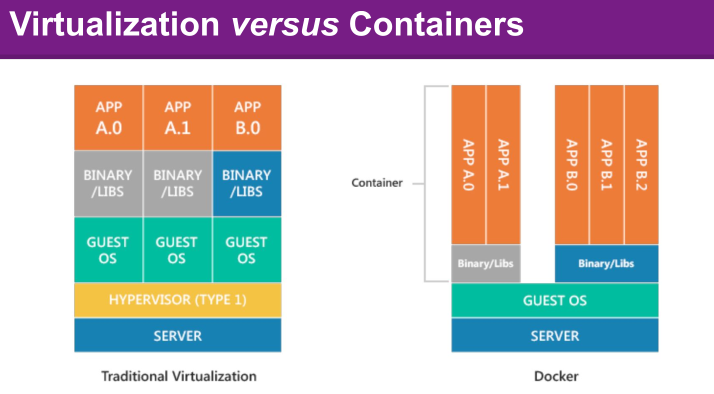
\includegraphics[width=0.8\textwidth]{img/contvsvirt.png}
    \caption{Confronto tra le macchine virtuali tradizionali e i container di Docker}
    \label{fig:docker_containerization}
\end{figure}

\subsection{Principali componenti}
\label{sec:principalicomponenti}

L’ecosistema Docker è composto da tre elementi principali:


\begin{itemize}
    \item \textbf{Software}: Il cuore del sistema è il Docker daemon (dockerd), un processo che gestisce i container e le altre risorse Docker. Gli utenti interagiscono con il daemon tramite il Docker Client, ovvero un'interfaccia a riga di comando (docker) che comunica attraverso le API di Docker Engine.
    \item \textbf{Oggetti}: Gli oggetti Docker rappresentano le entità fondamentali per il funzionamento delle applicazioni containerizzate. I principali sono:
    \begin{itemize}
        \item \textbf{Immagini}: template di sola lettura da cui vengono creati i container.
        \item \textbf{Container}: ambienti isolati in cui vengono eseguite le applicazioni.
        \item \textbf{Servizi}: permettono ai container di essere scalati su più Docker daemon creando così uno swarm (un insieme di di daemon cooperante tramite l'API di Docker).
    \end{itemize}
    Gli oggetti di Docker verranno trattati con maggiore dettaglio nelle seguenti sottosezioni.
    \item \textbf{Registry}: I registry sono archivi centralizzati dove vengono conservate le immagini Docker. Possono essere pubblici o privati; il più noto è Docker Hub, il registry predefinito. I registry permettono di caricare e scaricare immagini.
\end{itemize}


\subsection{Immagini e Dockerfile}
\label{sec:immaginiedockerfile}
Le applicazioni containerizzate in Docker vengono distribuite sotto forma di immagini Docker, ovvero template immutabili da cui si generano i container. Ogni immagine racchiude il file system e tutte le istruzioni necessarie per avviare l’applicazione all’interno di un container. La creazione di un’immagine è automatizzata tramite un file di configurazione testuale chiamato Dockerfile, in cui vengono specificati in modo dichiarativo tutti i passaggi necessari: dalla scelta dell’immagine di base (ad esempio una distribuzione Linux minimale), alla copia dei file dell’applicazione, fino all’installazione delle dipendenze e alla configurazione dell’ambiente (cartella di lavoro, utenti, variabili d’ambiente, ecc.). Questo approccio garantisce la riproducibilità e la coerenza dell’ambiente software, eliminando i tipici problemi di compatibilità tra sistemi diversi. Le immagini Docker possono inoltre essere versionate e facilmente condivise tramite i registry, favorendo la collaborazione e la distribuzione delle applicazioni.

\subsection{Container}
\label{sec:container}
Un container Docker è un’istanza attiva di un’immagine: rappresenta un ambiente isolato, leggero e portatile che esegue un’applicazione con tutte le sue dipendenze, come definito nell’immagine da cui è stato creato. Tuttavia, nella pratica, molte applicazioni moderne richiedono l’interazione tra più servizi distinti, ciascuno eseguito in un proprio container. Per gestire e orchestrare in modo semplice insiemi di container che compongono un’applicazione complessa si utilizza Docker Compose, uno strumento che permette di definire e avviare configurazioni multi-container tramite un unico file YAML.
Inoltre, poiché i container sono per loro natura effimeri e i dati scritti al loro interno vengono persi alla loro rimozione, Docker mette a disposizione i volumi: uno strumento pensato per garantire la persistenza dei dati e la condivisione delle informazioni tra container diversi o tra host e container.

\subsection{Docker Compose}
\label{sec:dockercompose}
Docker Compose è uno strumento che permette di definire, configurare e gestire applicazioni composte da più container. Tramite un file in formato YAML (docker-compose.yml), è possibile descrivere tutti i servizi che compongono l’applicazione, specificando per ciascuno l’immagine da usare, le variabili d’ambiente, le reti, le dipendenze e i volumi associati. Questo approccio consente di avviare, arrestare o aggiornare l’intero stack applicativo con un singolo comando, semplificando la gestione di architetture complesse e migliorando la riproducibilità degli ambienti sia in fase di sviluppo che di produzione. Compose è particolarmente utile quando si desidera far lavorare insieme più servizi (ad esempio un database, un’applicazione backend e un frontend), ciascuno eseguito nel proprio container ma coordinati tra loro.

\subsection{Volumi}
\label{sec:volumi}
I volumi in Docker rappresentano una soluzione per la persistenza dei dati nei container. Di default, i dati creati all’interno di un container sono temporanei e vengono eliminati quando il container viene rimosso. I volumi permettono di salvare dati in uno spazio dedicato e indipendente dal ciclo di vita dei singoli container, garantendo che le informazioni rimangano disponibili anche dopo la terminazione o la ricreazione dei container. Inoltre, i volumi possono essere utilizzati per condividere dati tra più container o per facilitare l’integrazione con il sistema host. Questa caratteristica è fondamentale per applicazioni che richiedono la conservazione dei dati, come database, sistemi di caching o storage di file.

Esistono due tipi di volumi:
\begin{itemize}
    \item \textbf{Bind Mount}: Consente di collegare una cartella o un file presente sul filesystem dell’host direttamente all’interno di uno o più container. Questo tipo di volume risulta particolarmente utile quando è necessario accedere a file specifici già esistenti o quando si dispone di spazio limitato sul disco gestito da Docker, poiché i dati vengono memorizzati direttamente nel percorso scelto sull’host.
    \item \textbf{Named Volume}: Si tratta di volumi gestiti direttamente da Docker, che vengono creati e organizzati in modo automatico dal Docker Engine all’interno di uno spazio dedicato dell’host. Sono ideali per la persistenza dei dati tra diverse esecuzioni dei container, e permettono una gestione più semplice e indipendente dal percorso fisico sul filesystem.
\end{itemize}

In generale, i bind mount sono consigliati quando si vuole controllare esattamente dove vengono salvati i dati o quando si ha poco spazio disponibile nell’area gestita da Docker, mentre i named volume offrono maggiore astrazione e portabilità nell’uso dei dati tra container diversi.




\section{Apache Airflow}
\label{sec:airflow}
Airflow è una piattaforma open-source progettata per la gestione automatizzata dei flussi di lavoro. Consente di definire, pianificare e monitorare in modo programmatico i workflow, tramite una pratica interfaccia utente integrata.
Creato originariamente da Airbnb, Airflow è sviluppato in Python ed è progettato secondo il paradigma del Configuration as Code. 

La Configuration-as-Code (CaC) è un approccio che prevede la gestione delle configurazioni tramite codice, invece che attraverso modifiche manuali o strumenti proprietari. In pratica, le configurazioni vengono trattate come vero e proprio codice applicativo. Questo metodo offre diversi vantaggi: garantisce coerenza e ripetibilità nelle configurazioni, riduce il rischio di errori umani e semplifica il ripristino in caso di problemi. Inoltre, essendo gestite come codice, le configurazioni possono essere versionate tramite sistemi di controllo versione (come Git), permettendo di tracciare facilmente le modifiche e tornare a versioni precedenti se necessario.

Airflow sfrutta Python per definire i flussi, a differenza di altre piattaforme simili, che tipicamente utilizzano linguaggi markup come XML. Questo approccio permette agli sviluppatori di importare librerie o script esistenti nel loro workflow.

Ogni workflow viene rappresentato come un DAG (Directed Acyclic Graph), ovvero un grafo orientato e aciclico, dove i nodi rappresentano i task (le singole operazioni da eseguire) e le frecce rappresentano le dipendenze e l’ordine di esecuzione tra i task.


\subsection{Concetti principali}
\label{sec:concettiprincipali}
Per comprendere il funzionamento di Apache Airflow, è fondamentale introdurre alcuni concetti chiave che costituiscono la base della piattaforma e ne determinano la logica operativa.

Tra questi i principali sono:
\begin{itemize}
    \item \textbf{DAG}: è la struttura fondamentale che descrive un workflow, ossia una sequenza di operazioni da eseguire secondo una precisa logica di dipendenze.
    Un DAG definisce quali task devono essere eseguiti e in quale ordine, rappresentando graficamente e logicamente il flusso di lavoro in cui ogni nodo è un task e ogni freccia una dipendenza. 
    Nel codice, un DAG è definito come un oggetto Python in cui si specificano parametri come:
    \begin{itemize}
        \item ID e descrizione del DAG;
        \item schedule\_interval (frequenza di esecuzione, ad esempio giornaliera o mensile);
        \item start\_date e altri parametri opzionali come ad esempio retries (quante volte può essere rieseguita una task);
        \item i task che lo compongono e le relative dipendenze (ad esempio, usando task1 >> task2).
    \end{itemize}
    
    La definizione di un DAG in Airflow consente di:
    \begin{itemize}
        \item Modellare pipeline di qualsiasi complessità,
        \item Visualizzare la struttura e lo stato delle esecuzioni tramite l'interfaccia grafica,
        \item Gestire in modo chiaro retry, fallback, e dipendenze tra task.
    \end{itemize}
    
    In seguito verrà mostrato un esempio di DAG:
    
    \begin{lstlisting}[language=Python]
    from airflow import DAG
    from airflow.operators.python import PythonOperator
    from datetime import datetime

    with DAG(
        dag_id="esempio_dag",
        start_date=datetime(2025, 1, 1),
        schedule_interval="@daily",
        catchup=False
    ) as dag:
        task1 = PythonOperator(
            task_id="primo_task",
            python_callable=lambda: print("Hello Airflow!")
        )
        task2 = PythonOperator(
            task_id="secondo_task",
            python_callable=lambda: print("Secondo task!")
        )
        task1 >> task2
    \end{lstlisting}
    
    \item \textbf{Task}: rappresenta l'unità base di esecuzione: ogni task corrisponde a una singola operazione o processo all'interno di un workflow. Le task vengono organizzate all'interno dei DAG e collegate tra loro tramite dipendenze che ne determinano l'ordine di esecuzione. 
    Esistono due principali tipi di task, nella mia implementazione ho utilizzato solo gli Operator ma li citerò per fornire un maggiore contesto:
    \begin{itemize}
        \item \textbf{Operator}: sono template di task predefiniti, pensati per svolgere operazioni comuni (ad esempio eseguire codice Python, eseguire comandi Bash, inviare email, ecc.). Sono il tipo di task più utilizzato. I principali sono PythonOperator, BashOperator, EmailOperator.
        \item \textbf{Sensor}: sono una sottoclasse di operator. Sono progettati per attendere il verificarsi di un evento esterno.
    \end{itemize}

    In Airflow, i concetti di Task e Operator sono in parte intercambiabili, ma è comunque utile pensarli come elementi distinti: in pratica, gli Operator e i Sensor rappresentano dei modelli (template), e ogni volta che ne istanzi uno all'interno di un DAG, stai effettivamente creando una Task.
    Ogni esecuzione di una task (detta Task Instance) attraversa diversi stati durante il proprio ciclo di vita:
    \begin{itemize}
        \item \textbf{none}: la task non è ancora stata messa in coda perché le dipendenze non sono soddisfatte
        \item \textbf{scheduled}: la task è stata programmata per l'esecuzione, avendo tutte le dipendenze soddisfatte
        \item \textbf{queued}: la task è in attesa di essere eseguita da un worker
        \item \textbf{running}: la task è in esecuzione
        \item \textbf{success}: la task è terminata con successo
        \item \textbf{failed}: la task è fallita a causa di un errore
        \item \textbf{skipped}: la task è stata saltata (ad esempio per una branch condizionale)
        \item \textbf{upstream\_failed}: una task a monte è fallita, impedendo l'esecuzione
        \item \textbf{up\_for\_retry}: la task è fallita, ma sono previsti tentativi di retry
        \item (altri stati specifici come restarting, up\_for\_reschedule, deferred, removed, etc.)
    \end{itemize}
\end{itemize}

\begin{figure}[h]
    \centering
    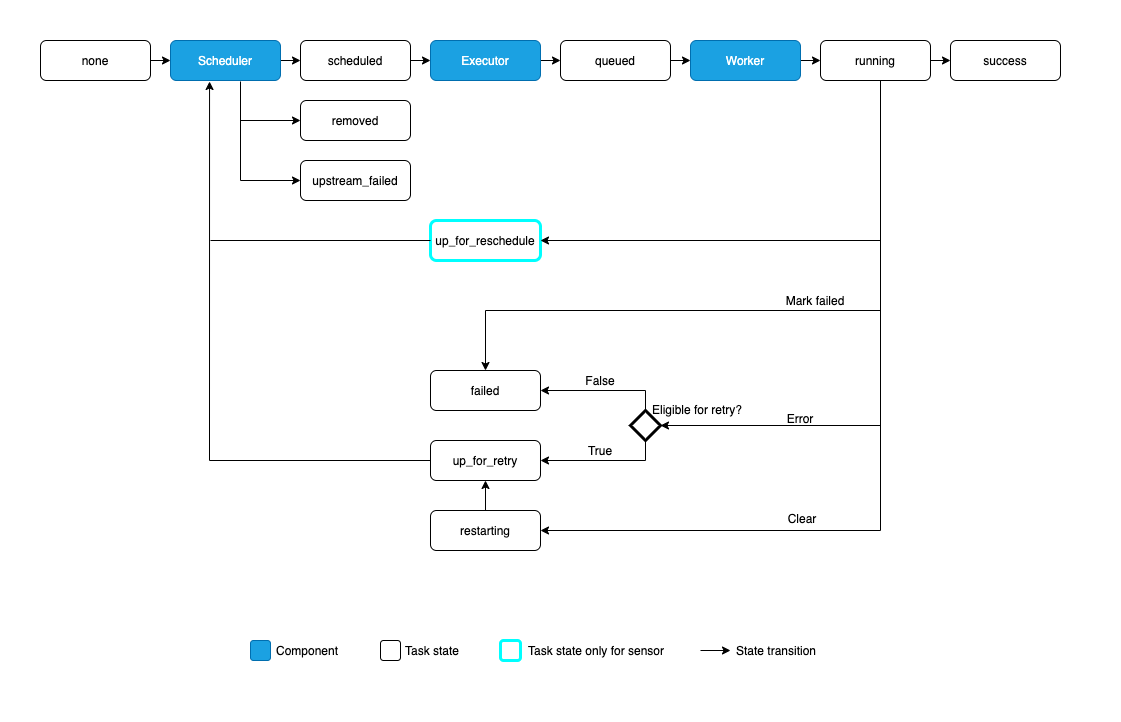
\includegraphics[width=0.8\textwidth]{img/task_lifecycle_diagram.png}
    \caption{Diagramma di tutti i possibili stati di una task}
    \label{fig:task_lifecycle}
\end{figure}

Come si può vedere in figura \ref{fig:task_lifecycle}, l'obiettivo ideale è che una task attraversi lo stato da none a success, passando per scheduled, queued e running. Per impostazione predefinita, una task viene eseguita solo se tutte le sue upstream (le task che la precedono nel flusso logico) sono completate con successo, ma Airflow offre anche strumenti avanzati di controllo del flusso (branching, trigger rules, ecc.).


\subsection{Architettura}
\label{sec:architettura}
L'architettura di Airflow è formata da diversi componenti. Un'installazione minima di Apache Airflow è formata in questo modo: 

\begin{itemize}
    \item \textbf{Scheduler}: Il cuore del sistema, si occupa di pianificare l'esecuzione dei workflow (DAG) secondo la programmazione definita, individuando i task che devono essere eseguiti e inviandoli all'esecutore (executor). L'executor, che è una proprietà configurabile dello scheduler, gestisce l'esecuzione dei task e può lavorare in modalità locale o distribuita, a seconda delle esigenze e delle risorse disponibili.
    \item \textbf{Webserver}: Fornisce un'interfaccia web intuitiva che permette di visualizzare, monitorare e gestire i DAG e i task, analizzare i log, forzare l'esecuzione manuale dei workflow e diagnosticare eventuali problemi.
    \item \textbf{Cartella /dags}: Una directory locale (o su storage condiviso) in cui risiedono i file Python che definiscono i DAG. Lo scheduler esegue periodicamente la scansione di questa cartella per individuare nuovi workflow o aggiornamenti ai workflow esistenti.
    \item \textbf{Meta Database}: Un database relazionale (tipicamente PostgreSQL o MySQL) utilizzato da tutti i componenti di Airflow per tracciare lo stato delle esecuzioni dei DAG e dei task, memorizzare configurazioni, cronologia delle esecuzioni, log degli errori e altri metadati fondamentali.
\end{itemize}

\begin{figure}[h]
    \centering
    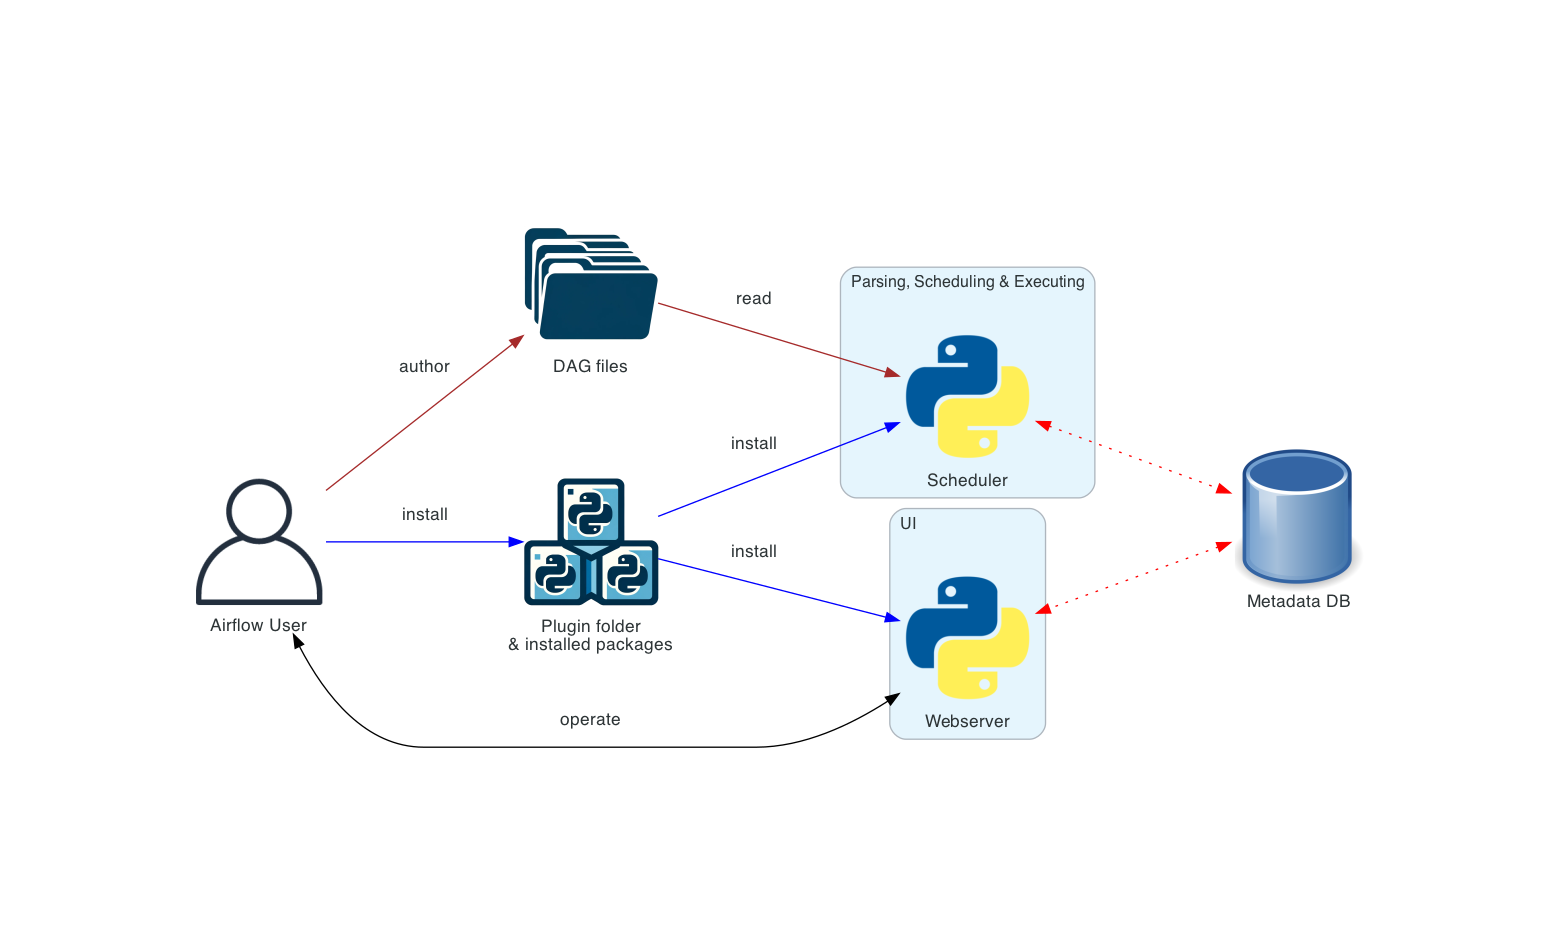
\includegraphics[width=0.8\textwidth]{img/diagram_basic_airflow_architecture.png}
    \caption{Fig 2.3 Diagramma del deployment minimo di Airflow}
    \label{fig:airflow_minimal_deployment}
\end{figure}

In figura ~\ref{fig:airflow_minimal_deployment} viene mostrata la configurazione più semplice di Airflow, in cui tutti i componenti principali (scheduler, webserver e database) vengono eseguiti sulla stessa macchina. In questo scenario si utilizza solitamente il LocalExecutor: scheduler e worker condividono lo stesso processo Python e i file dei DAG vengono letti direttamente dal filesystem locale. Anche l’interfaccia web (webserver) viene eseguita sulla stessa macchina. È importante far notare la differenza tra executor e worker: 
L’executor in Airflow determina la modalità e la logica con cui i task vengono messi in esecuzione, gestendo l’assegnazione dei task ai worker.
Il worker è invece il processo che riceve i task dall’executor e li esegue.

\subsection{Perché utilizzare Airflow?}
\label{sec:percheairflow}
Apache Airflow offre numerosi vantaggi nella gestione dei workflow. In primo luogo, la flessibilità della piattaforma consente di definire pipeline complesse come codice Python, integrandosi con praticamente qualsiasi tecnologia. Inoltre, l’automazione tramite la schedulazione integrata permette di eseguire i workflow a intervalli prestabiliti, e la gestione delle dipendenze garantisce che i task vengano eseguiti nell’ordine corretto secondo le relazioni definite. Airflow è altamente scalabile, potendo operare da un singolo processo locale fino a cluster distribuiti capaci di gestire carichi di lavoro ingenti. Offre anche un’ottima osservabilità: tramite un’interfaccia web si possono visualizzare chiaramente lo stato dei DAG, i log dei task e altri indicatori, facilitando il monitoraggio e il troubleshooting dei processi. Infine, sono previsti meccanismi di retry automatico e robusta gestione degli errori, così che eventuali fallimenti vengano intercettati e i task possono essere ritentati automaticamente per garantire la continuità delle pipeline.

\section{Monitoraggio e metriche}
\label{sec:monitoraggioemetriche}

Monitorare significa raccogliere, analizzare e visualizzare metriche e log per osservare il comportamento di un sistema nel tempo. Nell’ambito dell’informatica e dell’ingegneria del software, il monitoring si concentra principalmente sul tracciamento di metriche predefinite e indicatori chiave di performance (KPI) con l’obiettivo di rilevare deviazioni dal comportamento atteso.
Tipicamente vengono utilizzati strumenti di monitoring per raccogliere dati come utilizzo di CPU, memoria, tempo di risposta e tassi di errore. Questi dati vengono analizzati in tempo reale e, al superamento di determinate soglie, il sistema può inviare degli alert per consentire una risposta tempestiva a possibili problemi.

Nel mio progetto, il monitoring della pipeline dati è stato realizzato tramite l’integrazione di strumenti open source come StatsD, Prometheus e Grafana. Airflow esporta automaticamente metriche relative allo stato delle task, alle risorse utilizzate (CPU/RAM) e alla durata delle esecuzioni, che vengono poi raccolte e visualizzate in dashboard interattive. Questo consente di identificare rapidamente task fallite o anomalie di performance e intervenire in modo reattivo, garantendo affidabilità ed efficienza nella gestione dei workflow automatizzati.

\subsection{StatsD e StatsD Exporter}
\label{sec:statsd}

\textbf{StatsD} è un \textit{network daemon} sviluppato da Etsy, progettato per raccogliere metriche inviate dalle applicazioni tramite protocolli leggeri come UDP o TCP. Ogni metrica è rappresentata dalla sintassi:

\begin{verbatim}
<nome_metrica>:<valore>|<tipo>
\end{verbatim}

dove il nome, espresso in notazione a punti (es. \texttt{dag.task.duration}), identifica la metrica, il valore è numerico e il tipo può indicare un contatore (\texttt{c}), un gauge (\texttt{g}), un timer (\texttt{ms}), ecc. Airflow utilizza questo formato per esportare automaticamente informazioni come l’avvio e il completamento delle task, la durata delle esecuzioni e l’uso delle risorse, inviandole in modo asincrono e a basso overhead.

Poiché il formato StatsD non è compatibile con Prometheus, entra in gioco lo \textbf{StatsD Exporter}, un servizio che traduce le metriche ricevute in serie temporali etichettate secondo lo standard Prometheus. La conversione è definita tramite un file di mapping in YAML, che permette di trasformare un nome di metrica come:

\begin{verbatim}
task.cpu_usage.vital_signs.process_dump:30|g
\end{verbatim}

nella forma Prometheus:

\begin{verbatim}
cpu_usage{dag="vital_signs", task="process_dump"} 30
\end{verbatim}

In questo modo le metriche diventano interrogabili con PromQL e possono essere visualizzate in Grafana. Dal punto di vista infrastrutturale, StatsD Exporter è stato configurato come servizio dedicato in \texttt{docker-compose.yml}, in ascolto sulla porta \texttt{9125} per ricevere i pacchetti StatsD da Airflow e sulla porta \texttt{9102} per esporre le metriche convertite a Prometheus.

\subsection{Prometheus}
\label{sec:prometheus}
Prometheus è una piattaforma open source progettata per il monitoraggio e l’alerting. È nata in SoundCloud e oggi fa parte della Cloud Native Computing Foundation.
Il suo funzionamento si basa su un approccio pull: invece di ricevere metriche dagli applicativi, Prometheus interroga periodicamente gli endpoint degli strumenti monitorati (ad esempio ogni 5 o 10 secondi) e raccoglie le metriche esposte in un formato testuale standard.
Queste metriche vengono archiviate come serie temporali, cioè insiemi di valori numerici associati a un timestamp e a un insieme di etichette (labels) che ne descrivono il contesto, ad esempio il nome del task o l’identificativo del DAG in Airflow.

Prometheus offre diversi vantaggi:
\begin{itemize}
    \item conserva le metriche in un database ottimizzato per le serie temporali, permettendo query efficienti;
    \item utilizza un linguaggio dedicato, PromQL, che consente di analizzare e trasformare i dati (calcolare medie, percentili, confrontare valori tra task o host diversi);
    \item può generare regole di alerting, ad esempio inviando notifiche quando una metrica supera una certa soglia o quando un servizio non risponde più;
    \item si integra facilmente con strumenti di visualizzazione come Grafana, che permette di trasformare i dati raccolti in dashboard interattive.
\end{itemize}



      %\chapter{Risultati e Conclusioni}
\label{cha:risultaticonclusioni}

      
      
    \endgroup


    % bibliografia in formato bibtex
    %
    % aggiunta del capitolo nell'indice
    \addcontentsline{toc}{chapter}{Bibliografia}
    % stile con ordinamento alfabetico in funzione degli autori
    \bibliographystyle{plain}
    \bibliography{biblio}
%%%%%%%%%%%%%%%%%%%%%%%%%%%%%%%%%%%%%%%%%%%%%%%%%%%%%%%%%%%%%%%%%%%%%%%%%%
%%%%%%%%%%%%%%%%%%%%%%%%%%%%%%%%%%%%%%%%%%%%%%%%%%%%%%%%%%%%%%%%%%%%%%%%%%
%% Nota
%%%%%%%%%%%%%%%%%%%%%%%%%%%%%%%%%%%%%%%%%%%%%%%%%%%%%%%%%%%%%%%%%%%%%%%%%%
%% Nella bibliografia devono essere riportati tutte le fonti consultate 
%% per lo svolgimento della tesi. La bibliografia deve essere redatta 
%% in ordine alfabetico sul cognome del primo autore. 
%% 
%% La forma della citazione bibliografica va inserita secondo la fonte utilizzata:
%% 
%% LIBRI
%% Cognome e iniziale del nome autore/autori, la data di edizione, titolo, casa editrice, eventuale numero dell’edizione. 
%% 
%% ARTICOLI DI RIVISTA
%% Cognome e iniziale del nome autore/autori, titolo articolo, titolo rivista, volume, numero, numero di pagine.
%% 
%% ARTICOLI DI CONFERENZA
%% Cognome e iniziale del nome autore/autori (anno), titolo articolo, titolo conferenza, luogo della conferenza (città e paese), date della conferenza, numero di pagine. 
%% 
%% SITOGRAFIA
%% La sitografia contiene un elenco di indirizzi Web consultati e disposti in ordine alfabetico. 
%% E’ necessario:
%%   Copiare la URL (l’indirizzo web) specifica della pagina consultata
%%   Se disponibile, indicare il cognome e nome dell’autore, il titolo ed eventuale sottotitolo del testo
%%   Se disponibile, inserire la data di ultima consultazione della risorsa (gg/mm/aaaa).    
%%%%%%%%%%%%%%%%%%%%%%%%%%%%%%%%%%%%%%%%%%%%%%%%%%%%%%%%%%%%%%%%%%%%%%%%%%
%%%%%%%%%%%%%%%%%%%%%%%%%%%%%%%%%%%%%%%%%%%%%%%%%%%%%%%%%%%%%%%%%%%%%%%%%%
    

    \titleformat{\chapter}
        {\normalfont\Huge\bfseries}{Allegato \thechapter}{1em}{}
    % sezione Allegati - opzionale
    %\appendix
    %\input{allegati}

\end{document}
